\documentclass[../lecture-notes-148x210.tex]{subfiles}


\begin{document}

\subsection{Sum-Check-based Grand Product Protocol}
\label{sec:grand-products}

This subsection describes a transparent SNARK, which may be used for proving grand product relations of the following form:
\begin{equation}
\mathcal{R}_{GP} = \big\{ (p \in \mathbb{F}, \mathbf{v} \in \mathbb{F}^m)\colon p = \prod_{i=0}^m v_i \big\} \label{grand-product-relation}
\end{equation}
Without loss of generality, assume that $m$ is a power of $2$.
We can think of $\mathbf{v}$ as a vector of evaluations of a $\log m$-variate multilinear polynomial $v(x)$ over 
$\{0, 1\}^{\log m}$ in a natural fashion. We assume the prover first opens $p$ and then commits to $v(x)$; the 
following protocol then verifies both the polynomial’s validity and the corresponding grand-product equality derived
from that commitment.

\begin{lemma}
A scalar $p$ and a vector $\mathbf{v}$ satisfies the relation $\mathcal{R}_{GP}$ if and only if there exists a 
multilinear polynomial $f$ in $\log m + 1$ variables such that $f(1,\dots,1, 0) = p$ and $\forall x \in \{0,1\}^{\log m}$
 the following hold:
\begin{gather*}
f(0, x) = v(x)\\
f(1,x) = f(x, 0) \cdot f(x, 1)
\end{gather*}
Such polynomial $f$ has the following construction: \begin{itemize}
    \item $f(1,\dots,1) = 0$
    \item For all $\ell \in [\log m]$ and $x \in \{0,1\}^{\log m - \ell}$: \\ 
    \vspace{-0.8em}
    \begin{equation*}
        f(1^\ell, 0, x) = \prod_{y \in \{0,1\}^\ell}v(x,y)
    \end{equation*}
\end{itemize}
\end{lemma}

One can simply visualize the structure of $f$ as a binary tree.

\begin{example}
    Let $m=4$ ($\log m=2$), $\mathbf{v} = \{1, 2, 3, 4\}$, consequently $p = 1\times2\times3\times4=24$, then:
    \begin{align*}
    v(x_1, x_2)& = 1 + 2x_1 + x_2\\
    v(x_1,x_2)&: \quad v(0,0)=1,\; v(0,1)=2,\; v(1,0)=3,\; v(1,1)=4.
    \end{align*}
    Now, we define $f$ as follows:
    \begin{equation*}
        f(0,0,0)= 1,\; f(0,0,1)=2,\; f(0,1,0)=3,\; f(0,1,1)=4,
    \end{equation*}
    and:
    \begin{align*}
    f(1,0,0)&= f(0,0,0) \times f(0,0,1) = 1 \times 2 = 2,\\ 
    f(1,0,1)&= f(0,1,0) \times f(0,1,1) = 3 \times 4 = 12,\\ 
    f(1,1,0)&= f(1,0,0) \times f(1,0,1) = 2 \times 12 = 24 = p,\\ 
    f(1,1,1)&= 0.
    \end{align*}

    \begin{center}
        \scalebox{1.0}{
        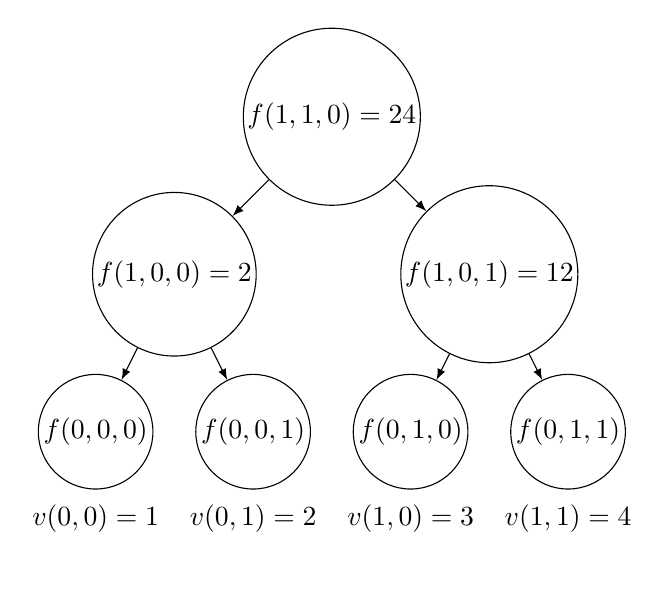
\begin{tikzpicture}[
            level 1/.style={level distance=2cm, sibling distance=4cm},
            level 2/.style={level distance=2cm, sibling distance=2cm},
            level 3/.style={level distance=1.1cm, sibling distance=2cm, edge from parent/.style={draw=none},},
            edge from parent/.style={draw, -latex},
            every node/.style={circle,draw,inner sep=1pt}
        ]
        \node {$f(1,1,0)=24$}
            child {
                node {$f(1,0,0)=2$}
                child { node {$f(0,0,0)$}
                    child { node[draw=none] {$\displaystyle v(0,0)=1$} }
                }
                child { node {$f(0,0,1)$}
                    child { node[draw=none] {$\displaystyle v(0,1)=2$} }
                }
            }
            child {
                node {$f(1,0,1)=12$}
                child { node {$f(0,1,0)$}
                    child { node[draw=none] {$\displaystyle v(1,0)=3$} }
                }
                child { node {$f(0,1,1)$}
                    child { node[draw=none] {$\displaystyle v(1,1)=4$} }
                }
            };
        \end{tikzpicture}
        }

        \vspace{-1em}
        \textit{\textbf{Illustration:} Binary tree of the Grand Product constraints for $v(x_1, x_2) = 1 + 2x_1 + x_2$.}
    \end{center}
\end{example}

Then, to check that $\forall x \in \{0,1\}^{\log m}$ the equation $f(1,x) = f(x, 0) \cdot f(x, 1)$ holds, we can use 
a sum-check protocol to prove the evaluation of $g$ that is referred to a MLE of $f(1,x) - f(x, 0) \cdot f(x, 1)$:
\begin{equation*}
    g(t) = \sum_{x \in \{0,1\}^{\log m}} \widetilde{\text{eq}}(t,x) \cdot (f(1,x) - f(x, 0) \cdot f(x, 1))
\end{equation*}
By the Schwartz–Zippel lemma, except for a soundness error of $\frac{\log m}{|\mathbb{F}|}$ (which should be negligible),
 $g(\tau) = 0$ for $\tau$ uniformly random in $\mathbb{F}^{\log m}$ if and only if $g = 0$, which implies that 
 $f(1, x) - f(x, 0) \cdot f(x, 1) = 0$ for all $x \in \{0, 1\}^{\log m}$.

Similarly, to prove that $v(x) = f(0, x)$ for all $x \in \{0, 1\}^{\log m}$ it suffices to prove that $v(\gamma) = f(0, \gamma)$
 for a public coin $\gamma \in \mathbb{F}^{\log m}$.

Thus, to prove the existence of $f$ and hence the grand product relationship, it suffices
to prove, for some verifier selected random $\tau, \gamma \in \mathbb{F}^\ell$, that:
\begin{gather}
\label{eq:grands0}
    0 = \sum_{x \in \{0,1\}^{\log m}} \widetilde{\text{eq}}(x, \tau) \cdot (f(1,x) - f(x, 0) \cdot f(x, 1))\\
\label{eq:grands1}
    f(0, \gamma) = v(\gamma)\\
\label{eq:grands2}
    f(1,\dots,1, 0) = p
\end{gather}
This can be achieved by running the sum-check protocol between $\mathcal{P}$ and $\mathcal{V}$, where $\mathcal{V}$ 
has oracle access to $v$ and $f$. Additionally, $\mathcal{V}$ evaluates the $f, v$ at the random point $\gamma$ to 
verify that $f(0, x) = v(x)$. So, the sum-check-based protocol for the grand products looks as follows:
\newline
\begin{algorithm}[H]
\caption{Sum-Check-based Protocol for Grand Products}\label{alg:sum_check_grand_product}
\DontPrintSemicolon
\SetAlgoLined

\textbf{$\mathcal P$:}
Compute polynomials 
$v\in\mathbb{F}^{\log m}[x]$, 
$f\in\mathbb{F}^{\log m+1}[x]$ 
such that
\vspace{-0.8em}
\begin{equation*}
    \vspace{-1.6em}
    p = \prod_{x\in\{0,1\}^{\log m}} v(x)
    \quad\text{and}\quad
    f, v \text{ satisfy }(\ref{eq:grands0}),\,(\ref{eq:grands1}),\,(\ref{eq:grands2}).
\end{equation*}\;

\textbf{$\mathcal P$:}
$C_f \leftarrow \textsc{Commit}(f)$;
$C_v \leftarrow \textsc{Commit}(v)$;
send $C_f, C_v$ to $\mathcal V$.\;

\textbf{$\mathcal V$:}
Choose random $\tau,\gamma\in\mathbb{F}^{\log m}$ and send them to $\mathcal P$.\;

\textbf{$\mathcal P$:}
Compute
\vspace{-0.8em}
\begin{equation*}
    \vspace{-1.6em}
    g(x)\;=\;\widetilde{\mathrm{eq}}(x,\tau)\,\bigl(f(1,x)-f(x,0)\,f(x,1)\bigr).
\end{equation*}\;

\textbf{$\mathcal P$ \& $\mathcal V$:}
Run \textsc{SumCheckProtocol}($0,\;g,\;C_f$)

\Comment{we assume this sum‐check runs over the commitment to $f$, not directly on $g$.}

\textbf{$\mathcal V$:}
$r \leftarrow \textsc{Query}(C_f,(1,\dots,1,0))$.\;
\If{$r \neq p$}{
    \textbf{$\mathcal V$ rejects}.\;
}

\textbf{$\mathcal V$:}
$a \leftarrow \textsc{Query}(C_f,(0,\gamma)), \;$ $v(\gamma)\leftarrow \textsc{Query}(C_v,\gamma)$.\;
\If{$a \neq v(\gamma)$}{
    \textbf{$\mathcal V$ rejects}.\;
}
\end{algorithm}

\begin{remark}
    Note, that during the call to the sum-check protocol, we pass the polynomial $g$ in a couple with the 
    commitment to $f$. Here we assume that each invocation of the \textsc{Query} method to $g$ inside the 
    sum-check instance will be more complex: \textbf{instead of evaluating a single function and returning 
    result, we evaluate $f$ at three different points, check the proofs and return results according to the
    construction of $g$}.
\end{remark}

\subsection{Randomized Permutation Check}
\label{sec:randomized-permutation-check}

The goal of the randomized permutation check is to verify, with high probability, whether two sequences
of tuples are permutations of each other, without performing a full sort or pairwise comparison.

\begin{definition}[Reed-Solomon Fingerprinting]
    Let $\mathbf{a} \in \mathbb{F}^{n}$, then for a random $\gamma \in \mathbb{F}$, the Reed-Solomon 
    fingerprinting of $\mathbf{a}$ is defined as:
    \begin{equation*}
        h_{\gamma}(\mathbf{a}) = \sum_{i \in n} a_i \cdot \gamma^i.
    \end{equation*}

    $h_{\gamma}(\mathbf{a})$ uniquely identifies the sequence $\mathbf{a}$ with high probability,
    i.e., let $\mathbf{b} \in F^n$ and $\mathbf{a} \neq \mathbf{b}$, then, according to the Schwartz-Zippel lemma:
    \begin{equation*}
        \Pr[h_{\gamma}(\mathbf{a}) = h_{\gamma}(\mathbf{b})] \leq \frac{n}{|\mathbb{F}|}.
    \end{equation*}
\end{definition}

\begin{definition}[Randomized Permutation Check]
    Let $A$ and $B$ be two multisets of tuples in $\mathbb{F}^n$. Define
    \begin{equation*}
        \mathcal{H}_{\tau,\gamma}(X)\;=\;\prod_{x \in X}\bigl(h_{\gamma}(x)-\tau\bigr).
    \end{equation*}
    Then comparing $\mathcal{H}_{\tau,\gamma}(A)$ and $\mathcal{H}_{\tau,\gamma}(B)$ yields a
    randomized test for whether $A$ and $B$ are permutations of one another. Concretely:
    \begin{itemize}
        \item (Completeness) If $A=B$ (as multisets), then  
            \begin{equation*}
                \mathcal{H}_{\tau,\gamma}(A)=\mathcal{H}_{\tau,\gamma}(B)
            \end{equation*}
            with probability 1 over uniform $\tau,\gamma\in\mathbb{F}$.
        \item (Soundness) If $A\neq B$, then
            \begin{equation*}
                \Pr\left[\,\mathcal{H}_{\tau,\gamma}(A)=\mathcal{H}_{\tau,\gamma}(B)\right]\;\le\; \frac{\max(|A|,|B|)}{|\mathbb{F}|}.
            \end{equation*}
    \end{itemize}
\end{definition}

In other words, by first “hashing” each tuple via the map function $h_{\gamma}$ and then taking the 
$\tau$‐shifted product, one obtains a fingerprint that is invariant under permutation but unlikely 
to collide on distinct sets.

\begin{example}
    Consider all operations in $\mathbb{F}_7$, and set $n=3$, $\tau=5$, and $\gamma=3$.  
    Let
    \begin{equation*}
      A = \{(1,2,3),\,(4,0,6)\}, \quad
      B = \{(4,0,6),\,(1,2,3)\},
    \end{equation*}
    First compute the Reed–Solomon fingerprints modulo 7:
    \begin{align*}
        h_{\gamma}(1,2,3) &=1\cdot3^0 + 2\cdot3^1 + 3\cdot3^2 =1 + 6 + 6 =13 \equiv 6,\\
        h_{\gamma}(4,0,6) &=4\cdot1 + 0\cdot3 + 6\cdot2 =4 + 0 + 12 =16 \equiv 2.
        \vspace{-5px}
    \end{align*}
    Now form the shifted products:
    \begin{align*}
        \mathcal{H}_{\tau,\gamma}(A) &=(6-5)\,(2-5) =1\cdot(-3)\equiv4,\\
        \mathcal{H}_{\tau,\gamma}(B) &=(2-5)\,(6-5) =(-3)\cdot1\equiv4,
    \end{align*}
    so the test \emph{accepts} $A$ vs.\ $B$ (they are indeed permutations). \\

    Now consider a non-permutation $B'$:
    \begin{equation*}
      B' = \{(1,2,3),\,(2,1,3)\}.
    \end{equation*}
    \begin{equation*}
      h_{\gamma}(2,1,3) =2\cdot1 + 1\cdot3 + 3\cdot2 =2 + 3 + 6 =11 \equiv 4.
    \end{equation*}
    \begin{equation*}
      \mathcal{H}_{\tau,\gamma}(B') =(6-5)\,(4-5) =1\cdot(-1)\equiv6\neq4,
    \end{equation*}
    so the test \emph{rejects} $A$ vs.\ $B'$.  
    In this way a single choice of $(\gamma,\tau)$ distinguishes permutations from non-permutations.
\end{example}

\subsection{Offline Memory Checking}
\label{sec:offline-memory-checking}

This protocol lets you, after doing a bunch of read/writes from an untrusted memory, verify in one quick
algebraic step that every answer really came from the same original contents -- without re-running any reads.

For the first time it's not so obvious, why we may need need such a protocol, so let's start with a simple 
example.
\begin{example}
    Consider Alice, who stores two values on Bob's dedicated server at addresses $0$ and $1$.  Initially, 
    Bob's memory contains
    \vspace{-5px}
    \begin{equation*}
      M \;=\;\{(0,100),\;(1,200)\}.
      \vspace{-5px}
    \end{equation*}
    Alice then performs the following operations in sequence:
    \begin{enumerate}
        \item Alice writes a new value $150$ at address $0$.  Bob updates his memory to $\{(0,150),(1,200)\}$.
        \item Alice reads from address $0$ and obtains the reply $150$.
        \item Alice reads from address $1$ and (honestly) obtains $200$.
    \end{enumerate}
    At this point, both replies individually look correct. However, Bob can cheat on the very last step by 
    returning, say, $300$ instead of $200$:
    \vspace{-5px}
    \begin{equation*}
      (1,200)\;\longrightarrow\;(1,300).
      \vspace{-5px}
    \end{equation*}
    Alice only sees the single read result ``$300$ at address $1$,'' which could simply be the true value 
    after some write she missed—and she has no immediate way to detect the inconsistency.\\ \\
    In other words, without keeping an auditable record of all reads, Alice cannot later prove that all 
    replies came from a single, immutable memory state.  This gap is exactly what an \emph{offline memory check}
    fills: after all reads are done, Alice runs one fast verification that guarantees “every read you saw really
    did come from one fixed initial memory + your writes,” and thus catches any cheating by Bob.
\end{example}

Each memory cell can be described as a tuple $\mathsf{(addr, val, counter)}$, where $\mathsf{addr}$ is the
address of the memory cell, $\mathsf{val}$ is the value stored at that address, and $\mathsf{counter}$ is the
number of times the memory cell has been accessed. You can think of a counter as a timestamp. The memory is
a vector of memory cels.

The protocol utilizes four sets of tuples:
\begin{itemize}
    \item $\mathbf{init}$ -- contains the initial memory state, where all counters are set to $0$;
    \item $\mathbf{write}$ -- contains memory cels that represent write operations, where $\mathsf{val}$
    is the value stored at the memory address $\mathsf{addr}$ after the specified counter;
    \item $\mathbf{read}$ -- contains memory cels that represent read operations, where $\mathsf{val}$
    is the value read from the memory address $\mathsf{addr}$ at the specified counter;
    \item $\mathbf{final}$ -- contains the final memory state, where all counters are set to the last value
    after the last read/write operation.
\end{itemize}

At the beginning, $\mathbf{init}$ is populated with the initial memory state, where all 
counters are set to $0$, indicating that the values were first accessed during the initialization phase, while
the $\mathbf{read}, \mathbf{write}$ are empty. Then, for each read operation, the untrusted memory is queried at 
$\mathsf{addr}$, returning a pair $\mathsf{(val, counter)}$, and writing a tuple $\mathsf{(addr, val, counter)}$ to the 
$\mathbf{read}$ set. For each write operation a corresponding tuple $\mathsf{(addr, newval, counter + 1)}$, where 
$\mathsf{newval}$ is a value being written, is added, with counter incremented by one, to the $\mathbf{write}$ set.

We assume that before each write operation, the read operation is performed. And the read operation is always followed 
by a write operation to the same address. Thus, to make a plain read operation, the prover first reads the value from 
the memory, then writes it back to the memory.

After all reads and writes are done, the $\mathbf{final}$ set is populated with the final memory state. Now, the
verifier can check the consistency of all the operations by verifying the following equation:
\begin{equation*}
    \mathbf{read} \cup \mathbf{final} = \mathbf{write} \cup \mathbf{init}.
\end{equation*}

Thus, using randomized permutation check, one can rewrite the equation as follows:
\begin{small}
\begin{align*}
    \mathcal{H}_{\tau,\gamma}(\mathbf{read}) \cdot \mathcal{H}_{\tau,\gamma}(\mathbf{final})& = 
    \mathcal{H}_{\tau,\gamma}(\mathbf{write}) \cdot \mathcal{H}_{\tau,\gamma}(\mathbf{init}),\\
    \prod_{(a,v,t)\in \mathbf{read}}\bigl(h_{\gamma}(a,v,t)-\tau\bigr) &\prod_{(a,v,t)\in \mathbf{final}}\bigl(h_{\gamma}(a,v,t)-\tau\bigr) = \\
    = \prod_{(a,v,t)\in \mathbf{write}}\bigl(h_{\gamma}(a,v,t)-\tau\bigr)& \prod_{(a,v,t)\in \mathbf{init}}\bigl(h_{\gamma}(a,v,t)-\tau\bigr), \\
    \prod_{(a,v,t)\in \mathbf{read}}\bigl((a\gamma^2+v\gamma+t)-\tau\bigr) &\prod_{(a,v,t)\in \mathbf{final}}\bigl((a\gamma^2+v\gamma+t)-\tau\bigr) = \\
    = \prod_{(a,v,t)\in \mathbf{write}}\bigl((a\gamma^2+v\gamma+t)-\tau\bigr)& \prod_{(a,v,t)\in \mathbf{init}}\bigl((a\gamma^2+v\gamma+t)-\tau\bigr).
\end{align*}
\end{small}

\begin{example}
\noindent Suppose the we track a single \emph{row-memory}, the algorithm performs three reads and two writes, 
the initial memory is given by the following table:
\begin{center}
    \centering
    \begin{tabular}{|c|c|c|c|c|}
        \hline
        Address & 0 & 1 & 2 & 3 \\ \hline
        Value   & 2 & 5 & 7 & 9 \\ \hline
    \end{tabular}
\end{center}

\medskip
\noindent\textbf{Initial memory (counter $0$):}
\begin{equation*}
\mathbf{init} =\{(0,2,0), \; (1,5,0), \; (2,7,0), \; (3,9,0)\},
\end{equation*}
while 
\begin{equation*}
    \mathbf{read} = \varnothing \quad \text{and} \quad \mathbf{write} = \varnothing.
\end{equation*}

\medskip
\noindent\textbf{Trace 1 - consistent execution}
\begin{center}
    \begin{tabular}{c|c|c|c}
    \textbf{step} & \textbf{operation} & $\Delta\mathbf{read}_{\text{step}}$ & $\Delta\mathbf{write}_{\text{step}}$\\\hline
    1 & read(1)$  \; \to \; (5, 0)$ & $(1,5,0)$ & -        \\
    2 & write((1,6))                & -         & $(1,6,1)$\\
    3 & read(2)$  \; \to \; (7, 0)$ & $(2,7,0)$ & -        \\
    4 & write((2,7))                & -         & $(2,7,1)$\\
    \end{tabular}
\end{center}
After the four steps
\begin{equation*}
    \begin{aligned}
        \mathbf{read} &= \{(1,5,0), \; (2,7,0)\},\\
        \mathbf{write} &= \{(1,6,1), \; (2,7,1)\}.
    \end{aligned}
\end{equation*}
And we can fill $\mathbf{final}$ as:
\begin{equation*}
    \mathbf{final} = \{(0,2,0), \; (1,6,1), \; (2,7,1), \; (3,9,0)\}
\end{equation*}
One can clearly see that $\mathbf{read} \cup \mathbf{final} = \mathbf{write} \cup \mathbf{init}$.
\begin{align*}
    \{(1,5,0), (2,7,0)\} &\cup \{(0,2,0), (1,6,1), (2,7,1), (3,9,0)\} = \\
    = \{(1,6,1), (2,7,1)\} &\cup \{(0,2,0), (1,5,0), (2,7,0), (3,9,0)\}
\end{align*}

\medskip
\noindent\textbf{Trace 2 - inconsistent execution}\\
Let the second reading return a wrong value -- $a$, instead of $5$. So, the new trace would look like:
\begin{center}
    \begin{tabular}{c|c|c|c}
    \textbf{step} & \textbf{operation} & $\Delta\mathbf{read}_{\text{step}}$ & $\Delta\mathbf{write}_{\text{step}}$\\\hline
    1 & read(1)$  \; \to \; (a, 0)$ & $(1,a,0)$ & -        \\
    2 & write((1,6))                & -         & $(1,6,1)$\\
    \end{tabular}
\end{center}
After the two steps
\begin{equation*}
    \begin{aligned}
        \mathbf{read} &= \{(1,a,0)\},\\
        \mathbf{write} &= \{(1,6,1)\},
    \end{aligned}
\end{equation*}
The verifier checks $\mathbf{read} \cup \mathbf{final} = \mathbf{write} \cup \mathbf{init}$:
\begin{align*}
    \{(1,a,0)\} &\cup \{(0,2,0), (1,6,1), (2,7,0), (3,9,0)\} \neq \\
    \neq \{(1,6,1)\} &\cup \{(0,2,0), (1,5,0), (2,7,0), (3,9,0)\}
\end{align*}
and \emph{rejects}.\\

Actually, no multiset $\mathsf{final}$ that depends on the valid values and addresses can 
reconcile them.
\end{example}

\end{document}

